\chapter{Dynamic Obstacle Avoidance}
\label{chapter:obstacle}

\section{Obstacle Detection}
\label{section:obstacle-detection}

\par Explain what is obstacle detection

\par what is needed for obstacle detection

\par the setup, both simulated and real 

\subsection{Hand Eye Calibration}

\par explicar o hand eye calibration

\subsection{Robot Self-Identification}

\par In a point cloud in order to detect obstacles, the points from the robot need to be identified and excluded form the point cloud

\par código de robot self identification

\par imagem das esferas a identificar o robot

\par imagem dos resultados

\subsection{Obstacle Identification}

\par now that the robot is identified and removed from the point cloud, the remaining points need to be processed

\par creation of a region of interest surrounding the robot with an X amount of distance

\par inside that region of interest, describe de 2 obstacle identification scenarios, one with simulated sphere obstacles, the other with real random obstacles

\par ros node that listens to camera, joints states, and publishes an array of obstacles

\par imagem dos resultados finais

\section{Potential Fields Method}
\label{section:pf-method}

\par explain what is the potential fields method

\subsection{Attraction}

\par Frist an offline trajectory is created, from a set of waypoints, then, the closest point to the robot is calculated, then the robtos follows the trajectory selection the 2 next poitns, making a mean out of those and calculating the global eef speed, which is the attraction vector

\subsection{Repulsion}

\par from the array of obstacles published by the obstacle node, a repulsion vector is calculated that is inversely proportional to the distance of the EEF to the object

\subsection{Controller}

\par using the attraction and repulsion vector, a global velocity vector is calculated and published which represents the final direction of the eef 

\section{Real Time Obstacle Avoidance}

\par Ros architecture showing all of the nodes working together to create obstacle avoidance

\begin{figure}[h]
    \centering
    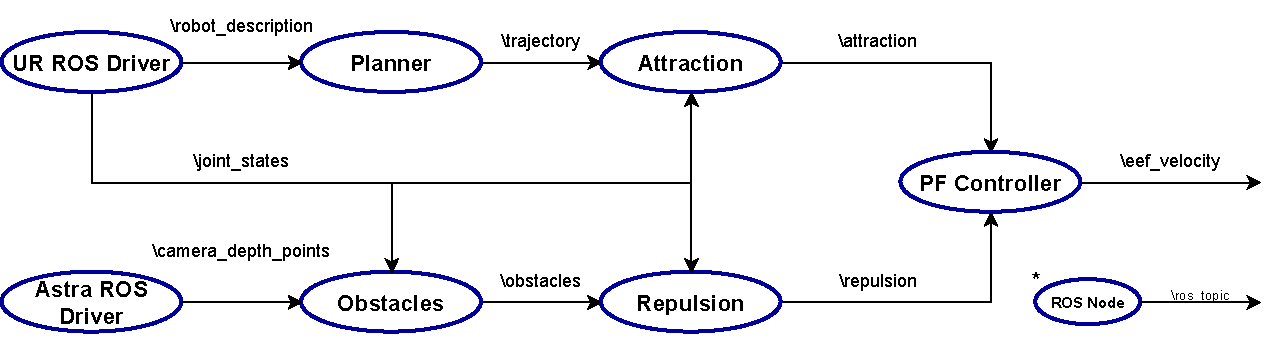
\includegraphics[width=\linewidth]{figs/chp4/ros_obstacle_arch.pdf}
    \caption{\ac{ros} architecture of the obstacle avoidance in real time}
    \label{fig:ros_obstacle_arch}
\end{figure}